\section{Digital Certificates}

\small



\begin{definition}{Digital Certificates}
A digital certificate is a signed statement by a trusted third party (Certificate Authority) that a certain public key belongs to a certain entity (person, organization, or system). Certificates are used to authenticate public keys, not the entities themselves.
\end{definition}

\mult{2}

\begin{concept}{Authentication of Public Keys}\\
The fundamental problem certificates solve is how to reliably distribute public keys in an insecure network:
\begin{itemize}
    \item Without certificates, it's difficult to know if a public key truly belongs to the claimed entity
    \item Certificates bind identities to public keys through the endorsement of a trusted third party
    \item The binding is authenticated through cryptographic signatures
\end{itemize}
\end{concept}



\begin{definition}{Certificate Types}

    \textbf{TLS Certificates}:

     Domain Validation (DV) - Validates domain ownership only

        Organization Validation (OV) - Validates domain ownership and organization details

        Extended Validation (EV) - Provides the highest level of validation

\textbf{Code signing certificates} - Authenticate software and files

\textbf{Client certificates} - Identify individual users or machines
\end{definition}

\begin{concept}{Public Key Infrastructure (PKI)}
PKI is the framework that manages digital certificates:
\begin{itemize}
    \item \textbf{Certificate Authorities (CAs)} - Issue and manage certificates
    \item \textbf{Registration Authorities (RAs)} - Verify identities before certificate issuance
    \item \textbf{Certificate stores} - Store trusted root certificates
    \item \textbf{Revocation systems} - Handle certificate invalidation
\end{itemize}
\end{concept}

\begin{definition}{X.509 Standard}
X.509 certificates are described in ASN.1 notation and typically encoded using DER (Distinguished Encoding Rules).
\end{definition}

\begin{concept}{X.509 Certificate Fields}

\textbf{Version} - Certificate format version (v1, v2, or v3)

\textbf{Serial Number} - Unique identifier assigned by issuing CA

\textbf{Signature Algorithm ID} - Algorithm to sign the certificate

\textbf{Issuer Name} - X.500 Distinguished Name of issuing CA

\textbf{Validity Period} - Start and end dates for certificate validity

\textbf{Subject Name} - X.500 Distinguished Name certif. owner

\textbf{Subject Public Key Info} - public key\& algorithm identifier

\textbf{Extensions} - Additional fields (e.g., key usage)

\textbf{Certificate Signature} - The digital signature created by CA

\end{concept}


\begin{definition}{Certificate Chains}
Certificates form chains of trust:
\begin{itemize}
    \item \textbf{End entity certificates} - Used by servers, clients, or devices
    \item \textbf{Intermediate CA certificates} - Issued by root CAs to intermediate CAs
    \item \textbf{Root CA certificates} - Self-signed certificates from trusted root authorities
\end{itemize}
To verify a certificate, each certificate in the chain must be validated up to a trusted root.
\end{definition}

\begin{concept}{Certificate Validation Process}
Certificate validation follows a simple chain of trust:
\begin{itemize}
    \item Each certificate's issuer must match the next certificate's subject
    \item Each certificate's signature must be verifiable by the next certificate's public key
    \item The chain must end with a trusted root certificate
    \item Certificate must be within its validity period and not revoked
\end{itemize}
\end{concept}

\begin{theorem}{Root Certificate Trust}\\
Root certificates are the foundation of trust in PKI:
\begin{itemize}
    \item Root certificates are pre-installed in operating systems and browsers
    \item They're the ultimate trust anchors that enable the validation of all other certificates
    \item The security of PKI depends on the protection of root CA private keys
\end{itemize}
\end{theorem}





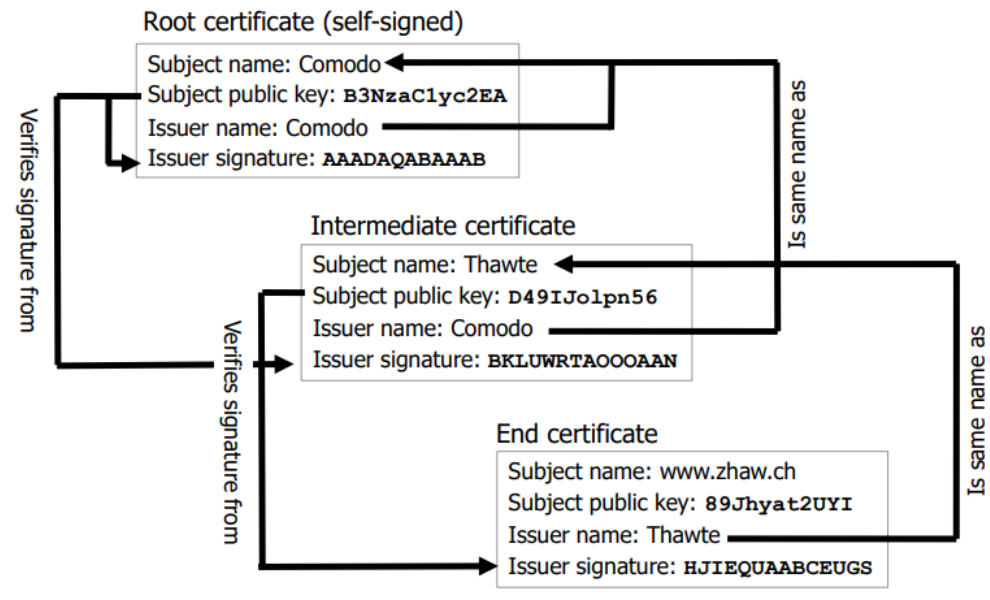
\includegraphics[width=\linewidth]{certificate_chain.png}

\multend









\subsubsection{Certificate Revocation and Transparency}

\mult{2}


\begin{definition}{Certificate Revocation}
     process of invalidating a certificate before its expiration date, typically due to:
\begin{itemize}
    \item Compromise of the associated private key
    \item Change in the certificate owner's status
    \item Cessation of operation by the certificate owner
\end{itemize}
\end{definition}

\begin{theorem}{Certificate Revocation Mechanisms}
\begin{itemize}
    \item \textbf{Certificate Revocation Lists (CRLs)} - Lists of revoked certificates published by CAs
    \item \textbf{Online Certificate Status Protocol (OCSP)} - Protocol for real-time certificate status checking
    \item \textbf{OCSP Stapling} - Server includes pre-fetched OCSP response during TLS handshake
    \item \textbf{OCSP Must-Staple} - Requires OCSP stapling for a certificate to be considered valid
    \item \textbf{Browser-Summarized CRLs} - Browser vendors compile and compress CRLs for distribution to browser instances
\end{itemize}
\end{theorem}

\begin{concept}{Revocation Checking Methods}
\begin{itemize}
    \item \textbf{CRLs}: Download revocation list from CA and check certificate serial number
    \item \textbf{OCSP}: Real-time query to CA for specific certificate status
    \item \textbf{OCSP Stapling}: Server pre-fetches OCSP response and includes it in TLS handshake
\end{itemize}
Each method has trade-offs between performance, privacy, and reliability.
\end{concept}





\begin{definition}{Certificate Transparency}
Certificate Transparency (CT) is a framework designed to detect and prevent the fraudulent issuance of certificates:
\begin{itemize}
    \item Publicly auditable logs of all issued certificates
    \item Monitors check logs for suspicious certificates
    \item Browsers require evidence that certificates are logged
    \item Helps detect malicious or mistakenly issued certificates
\end{itemize}
\end{definition}

\multend




